\documentclass[a4paper,zihao=5,UTF8]{ctexart}
\usepackage[top=2.3cm,bottom=2cm,left=1.7cm,right=1.7cm]{geometry} 
\usepackage{amsmath, amssymb}
\usepackage{color}
\usepackage{hyperref} 
\usepackage{pythonhighlight}
\usepackage{listings}
\usepackage{mathrsfs} 
\usepackage{booktabs}
\usepackage{amsthm}
\usepackage{longtable} 
\usepackage{graphicx}
\usepackage{subfigure}
\usepackage{caption}
\usepackage{fontspec}
\usepackage{titlesec}
\usepackage{fancyhdr}
\usepackage{latexsym}
\usepackage{subfigure}
\usepackage{braket}
\usepackage{cite}
\usepackage[version=4]{mhchem}
\usepackage{makecell}

\CTEXsetup[format={\Large\bfseries}]{section}
\def\d{\mathrm{d}}
\def\e{\mathrm{e}}
\def\i{\mathrm{i}}
\def\dps{\displaystyle}
\newcommand{\mr}[1]{\mathrm{#1}}
\newcommand{\mb}[1]{\mathbf{#1}}
\newcommand{\dv}[2]{\frac{\d{#1}}{\d{#2}}}
\newcommand{\pdv}[2]{\frac{\partial{#1}}{\partial{#2}}}
\def\degree{$^{\circ}$}
\def\celsius{^{\circ}\mr{C}}
\title{\textbf{实验六 \ce{Co(II)(Salen)}载氧体的制备及吸氧性质的测定}\cite{inorganic_chemistry_1}}
\author{王崇斌\;1800011716}
\makeatletter
\makeatother
\begin{document}
	\pagestyle{fancy}
	\pagestyle{fancy}
    \lhead{无机化学实验}
	\chead{}
	\rhead{\today}
	\maketitle
    \thispagestyle{fancy}

    \section{实验目的}
    \begin{enumerate}
        \item 通过钴载氧体的合成了解钴配合物分子氧配体的吸附和解附机制
        \item 通过对气体体积的测量了解理想气体状态方程的实际应用
    \end{enumerate}
    \section{实验原理}
    \subsection{载氧体}
    生物体内存在很多可以与分子氧形成配合物的包含过渡金属的蛋白质,在一定条件下可以可逆地
    吸附、释放氧气,以供生命活动的需要。例如,含铁的血红蛋白、肌红蛋白,含铜的血蓝蛋白等。
    其中血红蛋白与肌红蛋白是对大多数动物最为重要的载氧蛋白,其与分子氧配合的是蛋白质中
    的亚铁血红素,但是单独的亚铁血红素并不能可逆载氧\cite{comprehensive_inorganic_chemistry},
    在氧气中会被不可逆地氧化为高铁血红素,这说明蛋白质链的复杂结构在可逆载氧中同样起着
    重要的作用。生物无机化学家合成了很多类似的模型化合物进行相关研究,比较有代表性的
    是金属-西弗碱配合物与铁-卟啉配合物,通过调节金属离子和配体环上的取代基,人们希望探究
    影响载氧可逆性与载氧效率的因素,希望能够人工合成出高效的载氧体。

    \subsection{\ce{Co(II)(Salen)}配合物}
    \par Salen的结构如图\ref{Salen}所示,其由水杨醛和乙二胺缩合而成,
    是一种常用的四齿配体,通常占据八面体配合物的一个平面(因为其结构非常刚性)。
    \begin{figure}[htbp]
        \centering
        
\includegraphics[scale=0.15]{Preparation_of_salen.png}
        \caption{Salen的合成}
        \label{Salen}
    \end{figure}
    \par 
    由于制备方法的不同,\ce{Co(II)(Salen)}的固体可以以两种不同的形态存在,其中一种
    是暗红色胶冻状,可以在室温下迅速吸收氧气,因此称为活性型;另一种是暗红色结晶状固体,
    其在室温下稳定,不能吸收氧气,因此被称为非活性型。这两种不同形态的配合物结构不同,
    参见图\ref{CoSalen}。
    \begin{figure}
        \centering  
        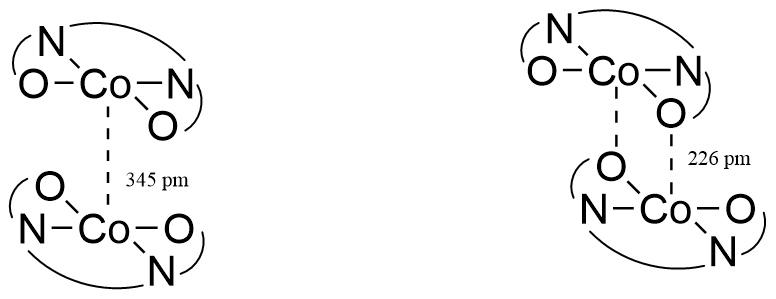
\includegraphics[scale=0.4]{CoSalen.png}
        \caption{活性配合物(左)和非活性配合物(右)}
        \label{CoSalen}
    \end{figure}
    \par 
    非活性的配合物可以在有一定配位能力的非质子溶剂L存在的情况下吸收环境中的氧气形成
    分子氧配合物\ce{[Co(II)(Salen)]L.O_2}和\ce{[Co(II)(Salen)]_2L_2.O_2},第二种
    配合物的结构如图\ref{[Co(II)(Salen)]_2L_2.O_2}所示。
    \begin{figure}
        \centering 
        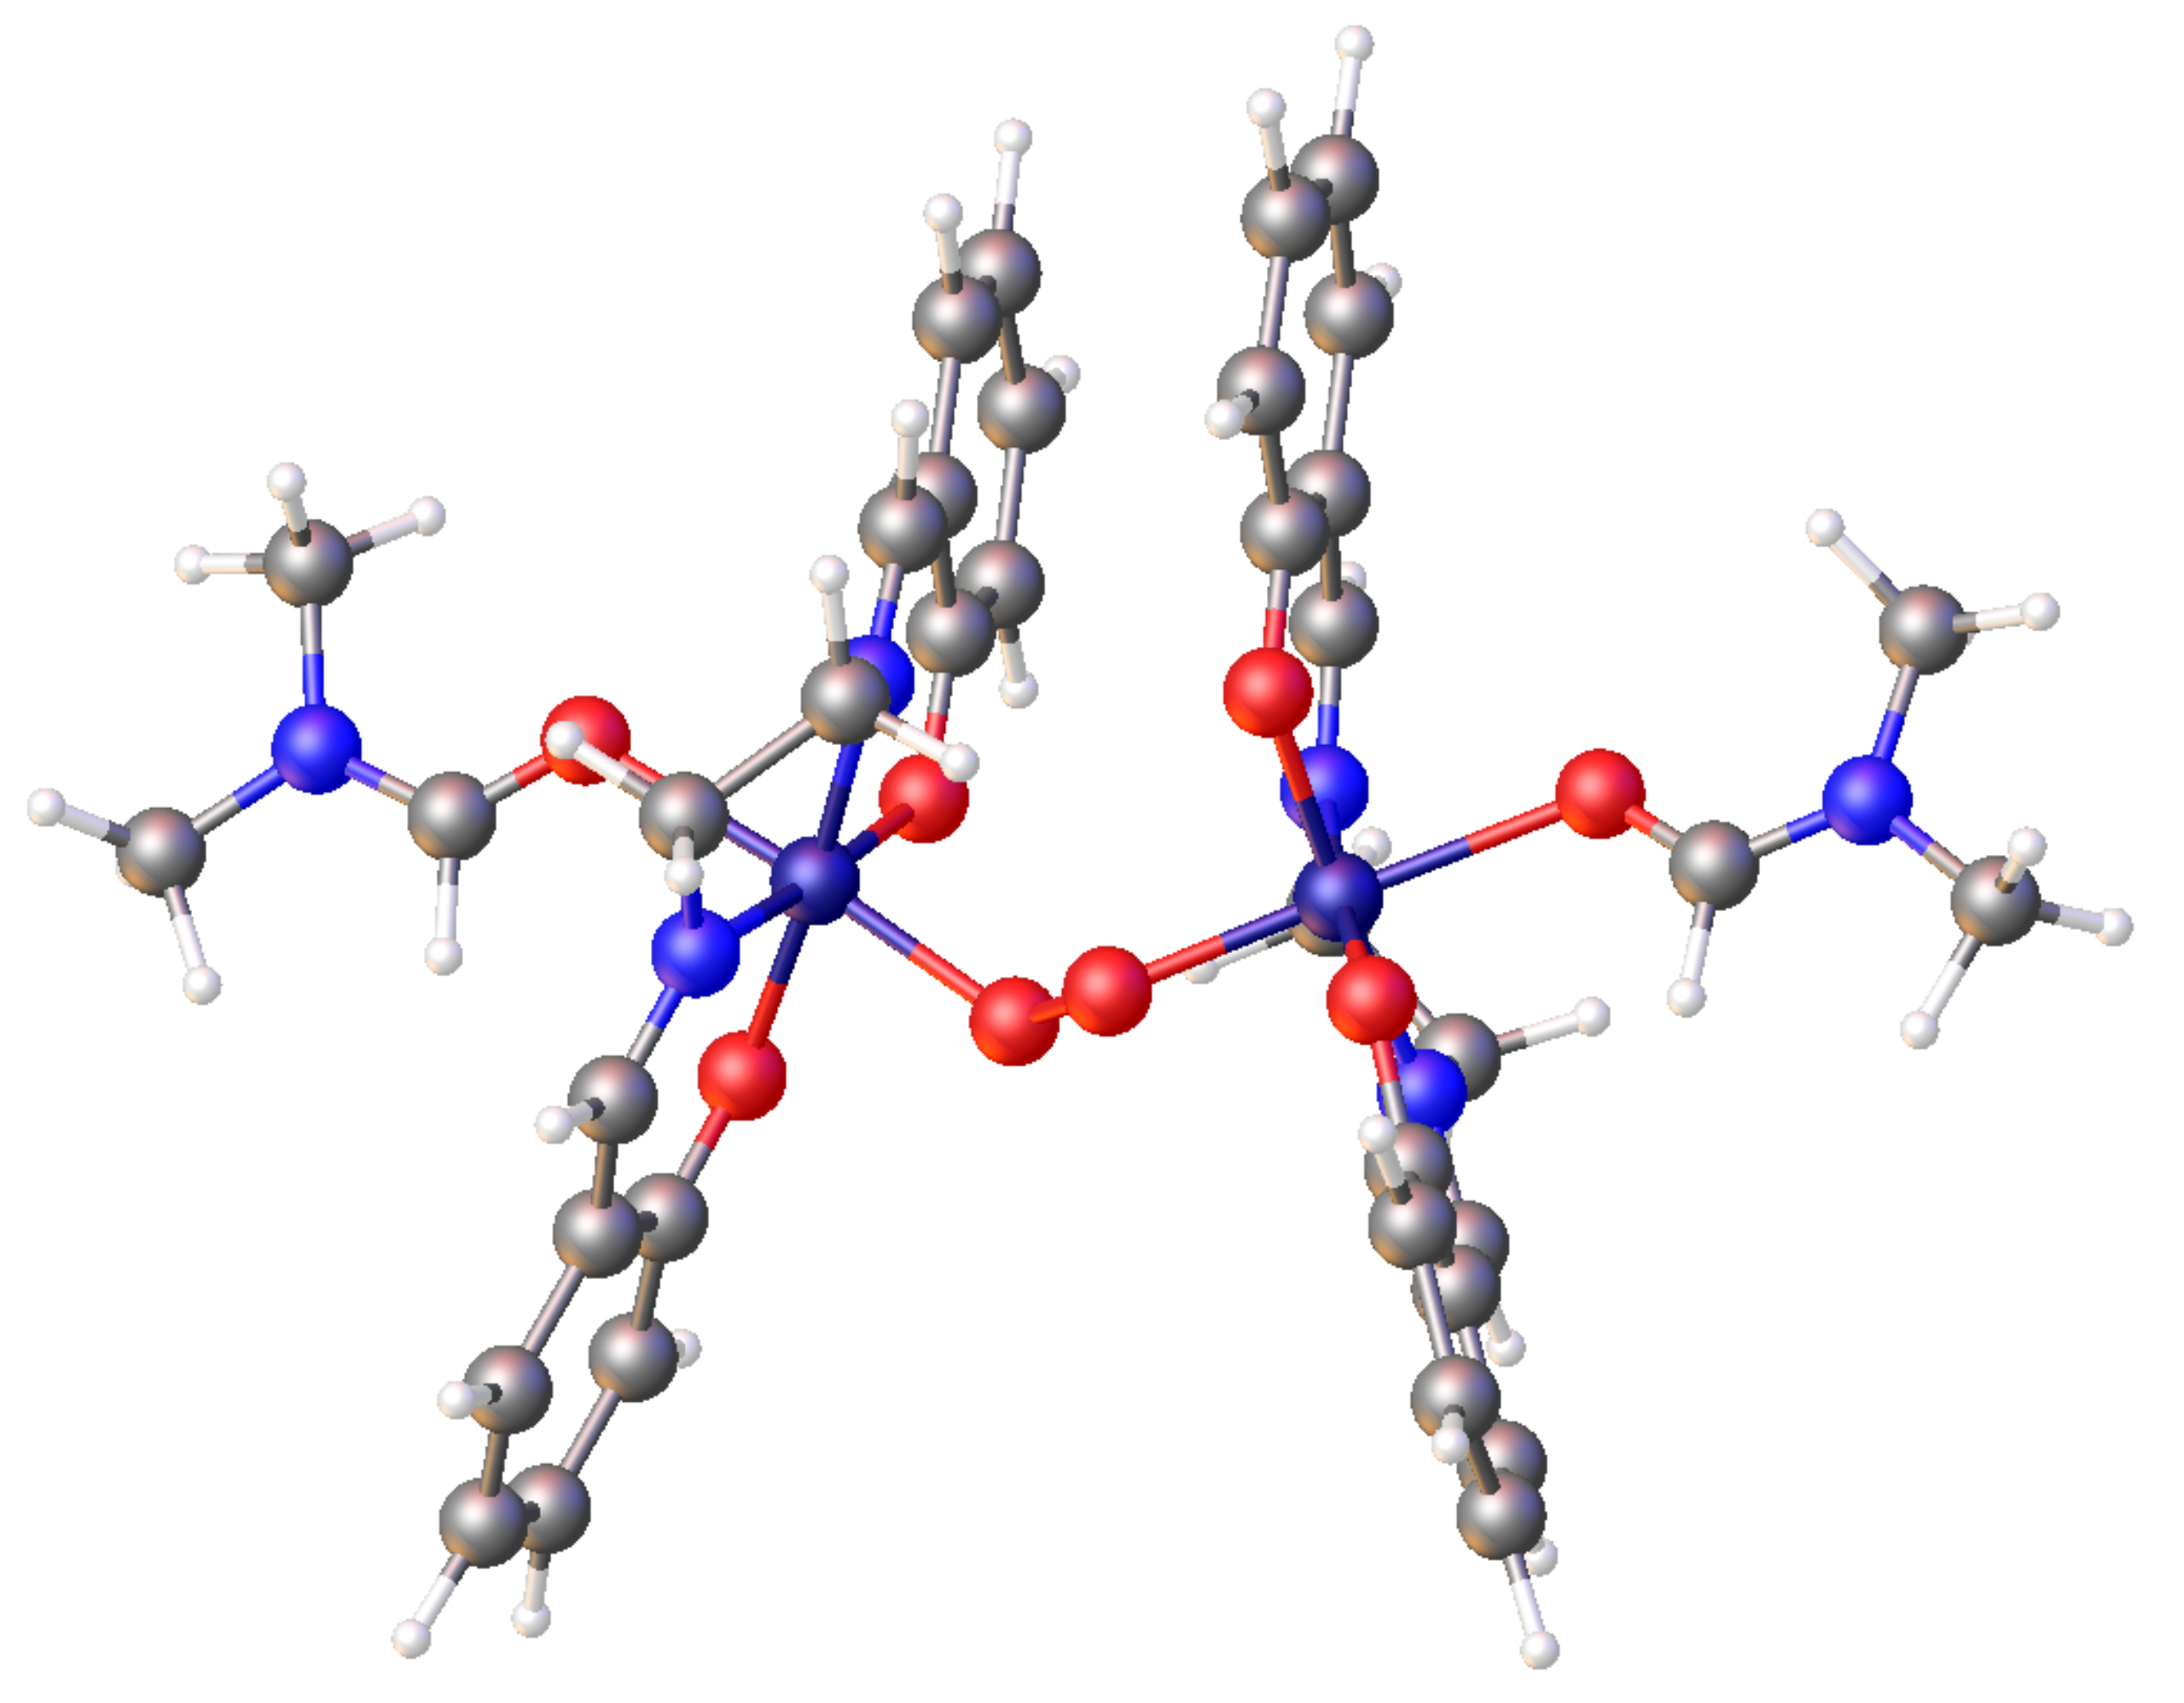
\includegraphics[scale=0.08]{Co2Salen2O2L2.png}
        \caption{\ce{[Co(II)(Salen)]_2L_2.O_2}的结构}
        \label{[Co(II)(Salen)]_2L_2.O_2}
    \end{figure}
    \par  
    配体L对于此配合物氧气的吸收是必须的
    \footnote{有可能L的存在使得$\mr{d}_{z^2}$
    轨道能量明显上升,存在于其上的单电子能量也上升,更易被氧化失去,但是
    由于\ce{Co(III)}有比较强的氧化性,此电子当配体的配位场强不足够强,
    也即分裂能不足够大时难以完全失去,因此表现为与氧配合。那么可以想象
    如果配体(主要指Salen)的配位场足够强以至于分裂能足够大(比如氨),此配合物很有可能
    容易被完全氧化,当配体的配位场强不足够,吸收氧就会变得困难}
    ,去除配体L会使得此配合物放出氧气,通常去除配体的方法为使用良溶剂
    将配体溶解(这是一个平衡过程),本实验会尝试使用多种不同的溶剂溶解,并比较实验现象。
    \section{实验过程及实验现象}
    \begin{enumerate}
        \item 实验地点:北京大学化学与分子工程学院D区三层第六实验室2号实验台
        \item 实验时间:2021年5月14日
    \end{enumerate}
    \subsection{制备非活性配合物\ce{Co(II)(Salen)}}
    在100mL烧杯中直接称取0.48g,1.9 mmol(0.4802g)
    \footnote{括号中为实验者实际称取的量,下同}
    \ce{Co(CH_3COO)_2.4H_2O},
    加入3.5mL去离子水溶解后吸入注射器备用。用1mL吸量管(移液枪)吸取0.40 mL
    ,3.8 mmol(0.40ml)水杨醛,移入100mL三口瓶,加入20 mL无水乙醇,摇匀。
    再用0.5 mL吸量管(移液枪)吸取0.125 mL,1.8mmol(0.125ml)乙二胺移入烧瓶
    (4~5min后溶液中产生黄色片状晶体)。在实验中实验者由于粗心没有留意讲义上的加料顺序
    ,将乙二胺和水杨醛同时先加入了三口烧瓶,随后加入了溶剂乙醇,在烧瓶中乙二胺和水杨醛
    混合的瞬间就生成了不规则的大块黄色固体,并放出热量,好在下一步中加热回流时
    固体完全溶解,并未对后续实验造成太大影响。
    \par 
    按图\ref{hechengzhuangzhi}搭好合成装置,开启搅拌,70~78℃水浴加热(保持回流)
    至黄色晶体全部溶解。经二通管向烧瓶通入氮气(液封处每秒1~2个气泡),
    5分钟后用注射器将醋酸钴溶液通过翻口塞缓慢滴加入三口烧瓶,10分钟加毕,水温维持在76℃左右。
    继续回流20分钟后,有大量暗红色晶状沉淀生成,溶液呈深棕黄色。
    停止加热,烧瓶用冰水浴冷却至室温,测量母液的pH(吸取少量母液加去离子水稀释后测量),
    首先用广谱试纸测得pH在4左右,而后用精密试纸测得pH=4.1。将沉淀转移至砂芯漏斗抽滤
    (不要用母液转移沉淀,但是我选择用去离子水转移沉淀),然后依次用5mL去离子水洗三次、
    1.5mL无水乙醇洗两次,再用1.5mL丙酮洗一次,抽干(洗涤过程不要搅动沉淀,
    是否是因为沉淀过于细密,搅动沉淀有可能极大地延长抽滤所需时间?)。
    产品转移到烘干称重的表面皿(m=38.2530g)中,称得此时的表面皿重量为38.69g(没有用分析天平
    称量,使用了实验室中的天平),100℃烘干1h,称得此时表面皿重量为38.6973g,可计算得到
    产物的质量为0.4443g。漏斗用6mol硝酸浸泡洗涤,并用大量水过滤洗涤后备用。
    \begin{figure}[htbp]
        \centering
        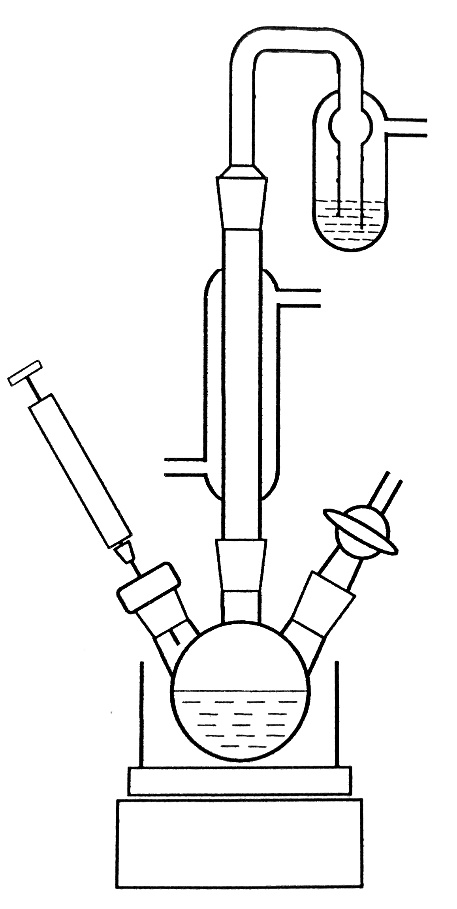
\includegraphics[scale=0.7]{hechengzhuangzhi.png}
        \caption{配合物的合成装置图示}
        \label{hechengzhuangzhi}
    \end{figure}
    \subsection{平衡液面法测定非活性配合物\ce{Co(II)(Salen)}的吸氧量}
    首先检查刻度量气管,不能有水珠挂壁,这个要在实验开始时提前检查并处理,
    装置各处接口涂凡士林。称取0.10~0.12g\ce{[Co(II)(Salen)]}通过干燥的漏斗
    转移至已经称重的干燥三口烧瓶(m=72.1534g)中,加入后三口烧瓶重m=72.2638g,
    增重$\Delta$m=0.1104g,n=0.339mmol。按图\ref{xiyangzhuangzhi}安装吸氧装置。
    \par 
    取5mL DMF于加料弯管中,将加料弯管与烧瓶连接,注意加料弯管的角度,防止溶剂被提前加入,
    用滴管向量气管中加1mL水形成液封。氧气袋充气后与活塞连接。
    \par 
	打开活塞,对氧气袋施压,鼓入氧气使空气通过刻度量气管排除,至氧气袋大部分气体被鼓入,
    关闭活塞。在刻度管加5mL水,如果液面在3分钟内变化小于0.03 mL
    (至少10分钟,以使体系热平衡),则认为装置气密性良好,并且体系已经达到热平衡,
    实验时液面的高度数据记录在表\ref{jianlougaodushuju}。
    如有漏气,检查各处接口并重复以上步骤。确认体系密闭性之后,打开活塞,使体系连通大气,
    当两管液面平齐时关闭活塞,记录液面刻度。
    \begin{table}[htbp]
        \caption{检漏时刻度量气管中的液面高度数据}
        \centering
        \label{jianlougaodushuju}
        \begin{tabular}[htbp]{cc}
            \toprule
            时刻(分:秒) & 液面高度(cm)\\
            \midrule
            00:00 & 5.07 \\
            04:00 & 4.97 \\
            12:00 & 4.94 \\
            17:00 & 4.92 \\
            \bottomrule
        \end{tabular}
    \end{table}
    \par
    确认不漏气后,
    转动加料弯管,加入DMF并快速搅拌,可以观察到紫红色配合物溶解,并迅速生成灰黑色胶状物质,
    同时刻度量气管中的页面迅速下降,这意味着配合物开始吸收氧气。与之同时并向量气管中补加水,
    维持两管液面相平。隔适当时间记录液面刻度,直至液面3分钟内变化小于0.03mL,记录最终液面刻度。
    作出体积随时间的变化曲线,并根据实验室气压和温度计算实际吸氧体积,此部分的记录参见后文
    讨论部分。
    \begin{figure}[htbp]
        \centering 
        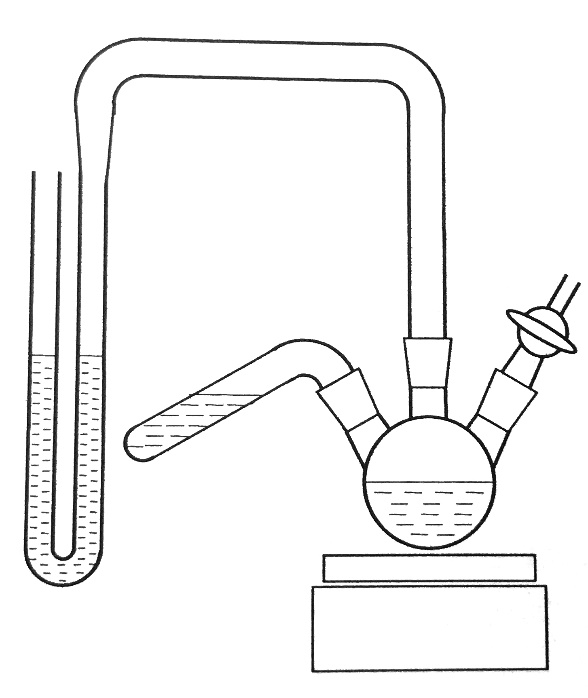
\includegraphics[scale=0.7]{xiyangzhuangzhi.png}
        \caption{吸氧装置图示}
        \label{xiyangzhuangzhi}
    \end{figure}
    \subsection{氧加合物\ce{[Co(II)(Salen)]_2L_2.O_2}在不同溶剂中氧的释放}
    把步骤2中生成的加合物转移至3只10mL离心管,2000r转速下离心5分钟,
    倾倒上层溶液至回收桶(尽可能分离掉溶剂)。保持试管倾斜,分别向三只离心管
    中加入4mL氯仿和2mL水(1)、
    4mL 1:1氯仿-无水乙醇和2mL水(2)、6 mL 50\%乙醇(3)。倾斜放置试管,不要搅动,观察现象。
    2~3分钟后,轻轻搅动观察现象,实验现象记录如表\ref{fenjieshiyanxianxiang}
    \begin{table}[htbp]
        \centering
        \caption{\ce{[Co(II)(Salen)]_2L_2.O_2}分解时的实验现象}
        \label{fenjieshiyanxianxiang}
        \begin{tabular}[htbp]{ccc}
            \toprule
            离心管编号 & 未搅拌 & 搅拌后 \\
            \midrule
            (1) & \makecell[c]{水与氯仿明显分层,氯仿相为橙色水相无色,\\有少量灰黑色配合物漂浮到
            相界面后缓慢产生气泡,\\气泡可以在两相交界处停留很长时间。}& 大量气泡在相界面生成\\
            (2) & \makecell[c]{氯仿与水+乙醇相之间的界面不明显,有很多液滴在两相间汇集\\
            氯仿相呈棕色,水+乙醇相呈现出淡黄色,\\气泡依然在两相间生成} & 气泡在两相间产生的速度明显加快\\
            (3) & \makecell[c]{加入瞬间溶液中迅速产生小气泡,随后溶液趋于稳定,\\ 
            溶液呈现出棕黄色} & 溶液中迅速生成大量细密气泡\\
            \bottomrule
        \end{tabular}
    \end{table}
    \section{结果与讨论}
    \paragraph{(1)}\textbf{计算合成反应产率}
    首先可以计算得到\ce{Co(II)(Salen)}的分子量为325.2g/mol,这样可以计算出产物中的钴的
    摩尔数为1.366mmol;四水合醋酸钴的相对分子质量为249.05g/mol,原料中的钴含量为1.935mmol,
    容易计算出产率为70.59\%。
    \paragraph{(2)}\textbf{测定吸氧量的试验记录}
    表 给出了刻度管内页面高度(补加水)随时间的变化关系。
    \begin{table}[htbp]
        \centering 
        \caption{吸氧时刻度量气管内页面随时间的变换}
        \begin{tabular}[htbp]{cc}
            \toprule
            时间(分:秒) & 液面高度(mL)\\
            \midrule
            00:00 & 3.30 \\
            00:30 & 4.45 \\
            01:00 & 6.20 \\
            01:40 & 7.40 \\
            02:20 & 7.45 \\
            05:00 & 7.50 \\
            08:00 & 7.56 \\
            11:00 & 7.60 \\
            12:00 & 7.60 \\
            14:00 & 7.60 \\
            \bottomrule
        \end{tabular}
    \end{table}
    可以认为最终的页面稳定在了7.60mL。
    \paragraph{(3)}\textbf{推到吸氧量$\Delta n$的计算公式和西弗碱钴的吸氧比率
    (\ce{O_2/Co}),写出吸氧和放氧过程的反应方程式}
    当时实验室内的温度为296K,气压为100.4kPa,
    由此可以计算出被吸收氧气的量为:
    \begin{equation}
        \mr{n}_\mr{O_2} = \frac{PV_{\mr{O_2}}}{RT} = 0.175\mr{mmol}
    \end{equation}
    那么容易计算出$\mr{n}_{\mr{Co}} : \mr{n}_{\mr{O_2}} = 1.94$。可以看出
    主要生成了图\ref{[Co(II)(Salen)]_2L_2.O_2}所示的配合物。那么吸氧和放氧的
    反应方程式可以写为:
    \begin{table}[htbp]
        \centering
        \begin{tabular}[htbp]{c}
            \ce{O_2 + 2Co(II)(Salen) + 2DMF -> [Co(II)(Salen)]_2DFM_2.O_2}\\
            \ce{[Co(II)(Salen)]_2DFM_2.O_2 + solvent -> O_2 + 2Co(II)(Salen) + 2DMF in solvent}\\
        \end{tabular}
    \end{table}
    \paragraph{(4)}\textbf{根据吸氧率分析吸氧产物的可能组成,如果吸氧率不是简单整数比
    分析可能的原因}
    可以看出主要生成了图\ref{[Co(II)(Salen)]_2L_2.O_2}所示的配合物。吸氧率并不是严格意义
    上的2:1,但是足够接近2:1,原因可能有2个,首先是非活性配合物以结晶的形式存在,有可能出现
    粘在烧瓶壁上没法充分反应的情况,其次有可能气体体积的测量并不准确,我认为这是实验误差的主要
    来源。影响气体体积测量的因素过多:温度变化,装置的气密性,加入水的过程中是否控制得当……这些都会
    导致气体体积测量有明显的误差。
    \section{思考题}
    \textbf{请用公式说明,采用左右液面高度差方法进行吸氧体积测量时,刻度量气管两边的
    页面对应的体积差是否就是吸氧体积?}
    \par 
    首先应该说明的是,量气管两边页面体积度数只差并不是吸氧体积,其至少应该对应2倍的吸氧体积。
    这就说明在使用液面高度差方法测量吸氧体积时,应当保证量气管内液体不能太少:吸气后最低液面处
    不能少于最小刻度;量气管内液体不能太多:吸气后最高液面处不能大于最大刻度。
    \par 
    假设使用高度差法达到平衡之后,记两边液面的高度差为h,大气压为$p_0$,在未混合之前,
    烧瓶内气体体积为$V$,刻度量气管两边液面差对应的体积为$\Delta V$,那么可以由下面一组
    方程给出吸收氧气的量:
    \begin{align}
        \Delta p = \rho_{H_2O}gh\\
        p_0V = nRT\\
        (p0 - \Delta p)(V - \frac{1}{2}\Delta V) = n'RT\\
        n_{O_2} = n - n'
    \end{align}
    \bibliographystyle{plain}
	\bibliography{ref}
\end{document}